%% Two Ways a Design Fails — CHI submission draft (acmart, sigconf).
%% Build: pdflatex main -> bibtex main -> pdflatex main -> pdflatex main
%% Figures are the vector PDFs in ../../figures/ (see \graphicspath).
%% Status: DRAFT v1 (2026-07-20). Numbers are audited (DECISIONS D5.20–D5.31).
%% Citations in references.bib are best-effort; entries marked "% VERIFY" need a metadata check.

\documentclass[sigconf,review,anonymous]{acmart}

%% --- ACM boilerplate (placeholder; fill for real submission) ---
\acmConference[CHI '27]{CHI Conference on Human Factors in Computing Systems}{April 2027}{Location}
\acmYear{2027}
\copyrightyear{2027}
\setcopyright{none}
\settopmatter{printacmref=false}
\renewcommand\footnotetextcopyrightpermission[1]{}
\pagestyle{plain}

\usepackage{booktabs}
\usepackage{graphicx}
\graphicspath{{../../figures/}}

\begin{document}

\title{Two Ways a Design Fails: When Does a Synthetic LLM Panel See the Danger?}

\author{Anonymous Author(s)}
\affiliation{%
  \institution{Anonymous Institution}
  \country{}
}

\begin{abstract}
Deploying an AI-advice interface can fail in (at least) two ways. It can make human reliance
\emph{heterogeneous and user-sensitive}---safe on average, dangerous for particular people (an
\emph{over-dispersion} failure). Or it can make users \emph{uniformly over-rely on a confidently wrong
AI}---a coercive \emph{dark-pattern} failure. Catching either normally requires an expensive human
study. A tempting shortcut is to screen an interface \emph{before} that study with a calibrated
multi-agent LLM panel that plays a synthetic cohort of users. We build such a panel---two-axis
(over-dispersion; wrong-AI over-reliance), conflict-conditioned, preregistered---and ask a question
prior to ``does it predict humans?'': \emph{are its danger signals even stable across the LLMs that
power it?} They are not. The signals are strongly \textbf{model-dependent}. On a guaranteed-wrong
interface, a frontier model (gpt-5.5) adopts the wrong advice only 15--30\% of the time---significantly
\emph{below} chance, i.e.\ it \emph{resists} the trap---and homogenizes cross-persona disagreement to
near zero, on two domains; other models show higher adoption, but idiosyncratically (only gpt-4.1
exceeds chance, and only after multiple-comparison correction on one of two domains). Independent-vendor
frontier models (claude-sonnet-4.5, gemini-2.5-pro) sit at chance. \textbf{The choice of panel model is
therefore a first-order, under-appreciated methodological decision: a single-frontier-model panel can
suppress a warning that other panel models raise.} Yet one signal is robust across all six models and
both domains: within the synthetic persona set, wrong-AI adoption \textbf{concentrates in a
trusting-novice persona}, the single most-susceptible profile in \textbf{12 of 12} model$\times$domain
cells (pooled odds ratio 15.0). The panel robustly ranks \emph{which persona} is most susceptible even
where aggregate rates do not transfer. We contribute (i) the model-dependence finding as direct evidence
for the silicon-sampling reliability debate, (ii) the persona-conditioned susceptibility invariant, and
(iii) the two-axis, over-dispersion-as-safety protocol; and we describe a preregistered, audit-gated
pipeline whose integrity is part of the method. We do \emph{not} claim to predict individual humans or a
validated deployment screen; we characterize \emph{when a synthetic panel does and does not see the
danger}, and design the human study that would ground it.
\end{abstract}

\begin{CCSXML}
<ccs2012>
<concept><concept_id>10003120.10003121</concept_id>
<concept_desc>Human-centered computing~HCI design and evaluation methods</concept_desc>
<concept_significance>500</concept_significance></concept>
<concept><concept_id>10010147.10010178</concept_id>
<concept_desc>Computing methodologies~Artificial intelligence</concept_desc>
<concept_significance>300</concept_significance></concept>
</ccs2012>
\end{CCSXML}
\ccsdesc[500]{Human-centered computing~HCI design and evaluation methods}
\ccsdesc[300]{Computing methodologies~Artificial intelligence}

\keywords{human--AI decision making, over-reliance, dark patterns, LLM simulation,
synthetic users, pre-deployment evaluation, silicon sampling}

\maketitle

\section{Introduction}

Consider a product team about to ship a review-triage tool. The interface shows an AI's verdict and a
confidence score and---to feel trustworthy---a highlighted ``explanation.'' Averaged over a pilot, the
numbers look fine: accuracy is up, users seem to like it. What the average hides is \emph{who} the
interface endangers and \emph{when}. A cautious domain expert barely moves; a \emph{trusting novice}
takes the AI's word almost every time---and if a coercive variant presents a confidently wrong verdict,
that same novice follows it off a cliff while the aggregate barely twitches. The design has not failed on
average. It has failed for a person, in a way the mean cannot see.

This is the gap between \emph{mean accuracy} and \emph{safety}. Two failure modes make it concrete---the
two ways a design fails in our title:
\begin{itemize}
  \item \textbf{Axis~1---over-dispersion.} Reliance becomes \emph{heterogeneous across users} in a way
  the interface induces. The team ships something safe for the median user and unsafe for the tails.
  Variance, usually a nuisance to be averaged away~\cite{bansal2021whole,gajos2022people}, is here the
  \emph{safety quantity of interest}.
  \item \textbf{Axis~2---wrong-AI over-reliance.} Under a coercive framing, users \emph{systematically
  adopt a wrong AI}. This is lethal even at zero dispersion: everyone fails
  together~\cite{bucinca2021trust,vasconcelos2023explanations,luguri2021shining}.
\end{itemize}

The standard way to detect either failure is a human-subjects study---powered, IRB-approved, and slow.
Teams iterate on interfaces far faster than they can run such studies. This paper asks whether a
\emph{cheap pre-deployment screen} can act like a smoke alarm: high-recall, run in minutes, flagging
interfaces that \emph{warrant} a human study and clearing those that plainly do not. Not a replacement
for the human study---a \emph{triage} in front of it.

The screen we investigate is a \textbf{calibrated synthetic panel}: persona-conditioned LLM agents that
role-play a cohort of users on the interface, from which we read the two axes directly. Synthetic users
are having a moment in HCI~\cite{park2022social,argyle2023out,aher2023using}, and so is the backlash: a
growing literature warns that LLM-simulated people are \emph{unreliable proxies}---they collapse human
diversity, echo the base model's priors, and mis-estimate distributions~\cite{santurkar2023whose,%
seshadri2026,cheng2023compost,hamalainen2023evaluating}. We take that critique seriously enough to ask a
question that comes \emph{before} ``does the panel predict humans?'': \textbf{is the panel's danger
signal even stable across the LLMs you might build it from?} If not, then any claim that ``the panel sees
the risk'' is really a claim about a particular model---and swapping the model can erase the warning.

Our central finding is that the danger signal is \textbf{strongly model-dependent}, and not in a tidy way
(Figure~\ref{fig:ladder}). On a guaranteed-wrong interface, the \emph{frontier} model we test (gpt-5.5)
does not fall for the trap---it adopts the wrong AI significantly \emph{below} chance and flattens
cross-persona disagreement to near zero, on \textbf{both} domains. Other models show higher adoption, but
\textbf{idiosyncratically}: the smallest model sits at chance, one mid-tier model (gpt-4.1) exceeds
chance, and two independent-vendor frontier models sit at chance. After multiple-comparison correction,
the only \emph{rock-solid} axis-2 regularity is gpt-5.5's cross-domain \textbf{resistance}; the
elevated-adoption effect is real but model-specific and survives correction on only one of two domains.
We interpret this association with capability cautiously---alignment, reasoning behavior, or training
could drive it as much as raw capability---but the practical upshot is robust: \textbf{the model you
choose to power a synthetic panel is a first-order methodological decision.} A team that screens with a
single frontier model may see a green light because \emph{that model} resists a coercion its less-capable
human users might not---a risk-masking failure mode we demonstrate \emph{within the panel} and
hypothesize (but do not yet show) for humans.

Against this negative, one result is stubbornly \textbf{robust} (Figure~\ref{fig:heatmap}). Even where the
model mean collapses, every model ranks the \emph{same} persona as most-susceptible: a
\textbf{trusting-novice} persona is the single highest-adopting persona in \textbf{12 of 12}
model$\times$domain cells (pooled odds ratio 15.0). The panel cannot tell you the \emph{rate} at which
people will over-rely---that depends on the model---but \emph{within its synthetic persona set} it robustly
ranks \emph{who} is most susceptible. We are careful: this persona is prompt-defined to be trusting, so
12/12 is in part consistent instruction-following; whether it maps to a real vulnerable human population is
an open question our planned study addresses.

We make three contributions, and we are explicit about their limits:
\begin{enumerate}
  \item \textbf{Model-dependence of synthetic-panel screening signals}---direct evidence for the
  silicon-sampling reliability debate: the \emph{same} preregistered protocol yields strong human-like
  failure signals on smaller/mid-tier models and has them resisted/homogenized by gpt-5.5, replicated
  across two domains. Panel-model choice is a first-order methodological decision that can, within the
  panel, suppress a warning other models raise.
  \item \textbf{A persona-conditioned susceptibility invariant robust across vendors}---even when the model
  mean collapses, the panel ranks the trusting-novice persona as most-susceptible (12/12 cells; sign-test
  $p=4.6\times10^{-10}$; pooled odds ratio 15.0). A synthetic-persona invariant scoped to relative
  \emph{ordering}, not aggregate rate, whose human validity is left to the planned study.
  \item \textbf{The two-axis protocol}---over-dispersion-as-safety plus wrong-AI over-reliance,
  conflict-conditioned and preregistered---proposed as a reusable \emph{testbed} for reasoning about
  interface-level reliance safety (not a validated screen), built on a preregistered, audit-gated pipeline
  whose process integrity (Section~\ref{sec:method}) is part of the method.
\end{enumerate}

We do \emph{not} claim a validated, model-agnostic detector, and we do \emph{not} claim to predict
individual humans. Our panel$\leftrightarrow$human correspondence is null in every configuration we can
currently test (all underpowered). We frame this as an open validation gap and describe the human study
(Section~\ref{sec:e6}) designed to close it.

\section{Related Work}

\paragraph{Simulated users, and the reliability critique.} LLMs as stand-ins for human participants have
been proposed for surveys, user studies, and formative
evaluation~\cite{park2022social,argyle2023out,aher2023using}. A parallel literature documents their
failure as proxies: they compress opinion diversity and over-represent majority
views~\cite{santurkar2023whose}, mis-calibrate distributions~\cite{seshadri2026}, and caricature rather
than simulate subpopulations~\cite{cheng2023compost,hamalainen2023evaluating}. We sit inside this debate
but change the target: we do not ask the panel to \emph{predict} a human distribution, we ask it to
\emph{triage} an interface, and we isolate a specific, measurable pathology---\emph{model-dependence of
the triage signal}---that the prediction framing obscures.

\paragraph{Reliance and over-reliance on AI advice.} A large body of work studies when people
appropriately rely on AI given confidence and
explanations~\cite{bansal2021whole,bucinca2021trust,zhang2020confidence,lai2019human,schemmer2023appropriate},
often finding explanations \emph{increase} over-reliance rather than calibrate
it~\cite{bansal2021whole,vasconcelos2023explanations}. This work treats between-user variance as noise
around an average. We invert that: reliance \emph{heterogeneity} is our axis-1 safety DV, and coercive
wrong-AI adoption is axis-2.

\paragraph{Dark patterns and coercive interfaces.} Deceptive and coercive designs are well
catalogued~\cite{luguri2021shining,mildner2023dark}; our axis-2 gives a computational signal for one
coercive mode (a confidently wrong AI) and, via personas, a read on \emph{who} it captures.

\paragraph{Offline evaluation of human--AI teams.} Closest is offline estimation of team performance for
decision support~\cite{rastogi2022deciding}; that work studies bias and complementarity, not
interface-level safety triage. The gap we fill is a \emph{pre-study screen for interface reliance safety},
and---critically---a characterization of when such a screen's signal is trustworthy.

\section{The Two-Axis Triage: Definitions}

We evaluate an interface $i$ on two axes, both measured on the panel's decisions.

\paragraph{Axis 1---between-user reliance over-dispersion.} For each item, personas produce reliance
decisions; we estimate the \emph{excess variance} beyond the binomial $p(1-p)$ a single homogeneous user
would produce (a beta-binomial over-dispersion estimator). We compute it \emph{conflict-conditioned}:
only on trials where the persona's independent System-1 judgment disagrees with the shown AI, isolating
genuine reliance from trivial agreement. High axis-1 means the interface makes reliance user-sensitive.

\paragraph{Axis 2---wrong-AI over-reliance.} Under a coercive ``dark'' framing, the interface shows a
\emph{guaranteed-wrong} AI verdict (the negation of ground truth) at high confidence. Axis-2 is the rate
at which personas adopt it. It is dangerous even at zero dispersion---a uniform failure.

\paragraph{The triage rule (design, not yet validated).} We learn thresholds $\tau_{\text{disp}},
\tau_{\text{level}}$ once in an atomic UI feature space; either axis over threshold $\Rightarrow$
\emph{recommend a human study}; both low $\Rightarrow$ \emph{release candidate}; out-of-distribution or
high-uncertainty $\Rightarrow$ \emph{abstain}. The rule is deliberately high-recall (a missed dangerous
interface is worse than a false alarm). We report it as a \emph{design}; its validation depends on the
human study (Section~\ref{sec:e6}), and thresholds remain unfrozen pending that study.

\section{Method: The Calibrated Synthetic Panel}
\label{sec:method}

\paragraph{Panel $=$ personas $\times$ models.} Each agent is a persona (a vector of domain skill, AI
literacy, risk sensitivity, caution) crossed with a base LLM. Personas span novice/expert $\times$
trusting/skeptical plus two moderates (six in total).

\paragraph{Dual-system decisions.} Each agent first produces a \textbf{System-1} judgment \emph{without}
AI (a frozen, no-AI anchor), then a \textbf{System-2} decision \emph{with} the AI advice and framing.
Reliance is defined against the System-1 anchor---what makes conflict-conditioning possible and prevents
the ``everyone-agrees-so-everyone-complies'' collapse of a naive panel.

\paragraph{Faithful interface rendering.} We reproduce the Bansal et al.~\cite{bansal2021whole}
explanation conditions faithfully (confidence-only; single/double highlighted-token explanations; adaptive
and expert-adaptive), and construct the dark condition by negating ground truth at high confidence. A
placebo condition (AI present, non-coercive) isolates coercion from mere AI-presence.

\paragraph{Stimuli and domains.} Items are drawn from the Bansal sentiment benchmark, held out from any
threshold fitting, and selected to concentrate on loci of human reliance heterogeneity (disclosed; human
outcomes are used only for \emph{item selection}, never leaked into agent prompts---item selection $\ne$
label leakage). We run two domains: \textbf{beer reviews} and \textbf{Amazon book reviews (amzbook)}.

\paragraph{Models.} A within-provider capability ladder (gpt-4o-mini $\to$ gpt-4.1 $\to$ gpt-4o $\to$
gpt-5.5, identical config) plus independent-vendor frontier models (claude-sonnet-4.5, gemini-2.5-pro):
six models total.

\paragraph{Rigor spine and process integrity.} The analysis was preregistered and frozen with UTC
timestamps before results; correspondence analyses were coded blind; every merge was gated on an
independent audit \emph{and} a from-raw numeric re-derivation. This spine caught three silent-corruption
bugs that would each have produced a plausible-but-false result: an axis-2 \emph{sign inversion} (scoring
adoption against \texttt{ground\_truth} instead of the displayed $1-\texttt{ground\_truth}$), a
beta-binomial \emph{boundary artifact}, and a decision parser that silently \emph{fabricated} a
$(\text{decision}{=}0,\text{conf}{=}0.5)$ sentinel on parse failure. We report these openly: for a paper
whose headline includes a negative and a nuanced positive, a pipeline that catches its own errors is what
makes the numbers trustworthy.

\section{Experiments and Results}

We report per-model (no pooling across incomparable models), with effect sizes, confidence intervals, and
Benjamini--Hochberg (BH) correction across the per-model test family. There are $n=120$ dark-condition
trials per model$\times$domain cell (6 personas $\times$ 20 items).

\subsection{Real human over-dispersion exists (anchor)}
On the Bansal human data, conflict-conditioned reliance over-dispersion is real and excludes zero
($\rho \approx 0.067$); no-AI reliance behaves as a stable trait ($\approx 0.74$) while AI-assisted
reliance is a user$\times$task interaction (0.32--0.41). This anchors axis-1 as a measurable human
quantity---and, honestly, does not generalize to a second human dataset (Lu \& Yin), which we report as a
boundary.

\subsection{The danger signal is model-dependent}
\label{sec:modeldep}

\begin{figure}[t]
  \centering
  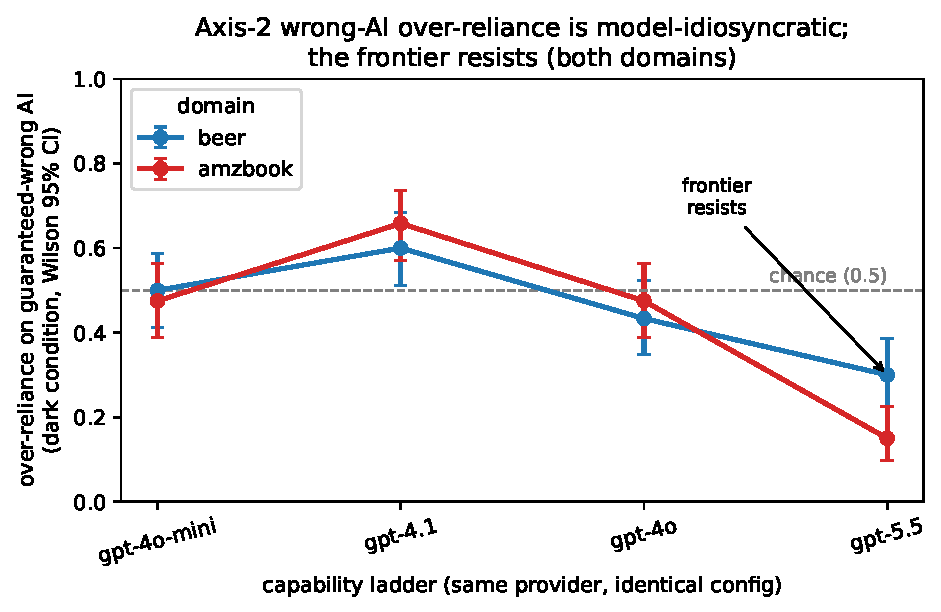
\includegraphics[width=\columnwidth]{fig1_axis2_ladder}
  \caption{Axis-2 wrong-advice adoption on the guaranteed-wrong interface across the same-provider
  capability ladder, both domains (Wilson 95\% CIs; dashed line $=$ chance). Adoption is non-monotonic
  and idiosyncratic; the frontier model (gpt-5.5) sits significantly \emph{below} chance on both
  domains---it resists.}
  \label{fig:ladder}
\end{figure}

On the guaranteed-wrong interface, axis-2 wrong-advice adoption is \emph{not} a clean function of
capability (Figure~\ref{fig:ladder}). Across the ladder (beer / amzbook): gpt-4o-mini 0.50 / 0.48, gpt-4.1
0.60 / \textbf{0.66}, gpt-4o 0.43 / 0.48, gpt-5.5 \textbf{0.30 / 0.15}. The frontier model is \emph{below}
chance on both domains (binomial BH $p=8\times10^{-5}$ beer, $2\times10^{-14}$ amzbook)---it resists
following the wrong advice. The adoption peak at gpt-4.1 is real (between-model Fisher vs.\ gpt-4o
$p=0.014/0.006$) but \textbf{model-idiosyncratic}: the smallest ladder model sits at chance, and after BH
correction gpt-4.1's elevated adoption survives on amzbook ($p=0.003$) but is only nominal on beer
(uncorrected $p=0.035$; BH $p=0.11$). Independent-vendor frontier models replicate the \emph{at-chance}
pattern, not the elevated adoption: claude 0.49, gemini 0.53 on beer (0/3 vendors exceed chance).

Axis-1 tells a parallel story more cleanly (Figure~\ref{fig:collapse}). Mean panel disagreement across the
ladder is 0.11 / 0.16 / 0.10 / \textbf{0.012} (beer) and 0.12 / 0.19 / 0.11 / \textbf{0.015} (amzbook):
gpt-5.5 collapses to near-homogeneity on both domains. This is not a no-conflict artifact---genuine
conflict trials remain present (e.g., 215/600 on amzbook)---the model \emph{resists diverging}.

\begin{figure}[t]
  \centering
  
\includegraphics[width=\columnwidth]{fig3_axis1_collapse}
  \caption{Axis-1 mean panel disagreement across the ladder, both domains. Heterogeneity collapses at the
  frontier (gpt-5.5) on both domains.}
  \label{fig:collapse}
\end{figure}

\emph{Coercion vs.\ mere advice-following (a caveat).} We measure adoption of a guaranteed-wrong AI against
chance; our data do not isolate the \emph{coercive framing} from ordinary wrong-advice following, because
we do not report the dark-vs-placebo contrast here (an immediate follow-up). We therefore describe axis-2
as \emph{wrong-advice adoption under a guaranteed-wrong stress test}, and reserve ``dark-pattern
susceptibility'' for the controlled contrast.

\paragraph{Reading.} gpt-5.5's cross-domain \textbf{resistance} (both axes) is the rock-solid regularity;
adoption magnitude is model-specific. A synthetic panel's aggregate reading is therefore a property of the
panel's model as much as of the interface: swapping in the frontier model can flip a warning to a green
light \emph{within the panel}.

\subsection{One signal is robust: which persona the panel ranks highest}

\begin{figure*}[t]
  \centering
  
\includegraphics[width=\textwidth]{fig2_persona_heatmap}
  \caption{Persona $\times$ model wrong-advice adoption on the dark condition, both domains. The
  trusting-novice persona (p5, highlighted) is the single highest-adopting persona in all 12
  model$\times$domain cells.}
  \label{fig:heatmap}
\end{figure*}

The aggregate adoption \emph{rate} is model-idiosyncratic (range 0.30 across beer models, 0.51 across
amzbook models). The \emph{ordering} of which persona adopts most is not (Figure~\ref{fig:heatmap}). A
\textbf{trusting-novice} persona is the single highest-adopting persona in \textbf{12 of 12}
model$\times$domain cells (sign-test vs.\ a $1/6$ chance top $p=4.6\times10^{-10}$). A pooled GEE logistic
regression (clustered by cell) gives an odds ratio of \textbf{15.0} (95\% CI 5.8--38.8,
$p=2\times10^{-8}$) for that persona adopting the wrong AI relative to the others; a per-cell Fisher test
is significant in \emph{all 12} cells after BH (largest BH $p=0.002$). The persona-minus-others adoption
gap is $+0.53$ on average and never below $+0.30$---it holds even at the resistant frontier. We foreground
the descriptive 12/12 and the large effect sizes over the $p$-values, whose inferential unit (12 cells
sharing prompts, items, and providers) is not fully independent; the persona is also prompt-defined to be
trusting, so this is best read as a \emph{robust synthetic-persona invariant} rather than established
human-population localization.

\begin{figure*}[t]
  \centering
  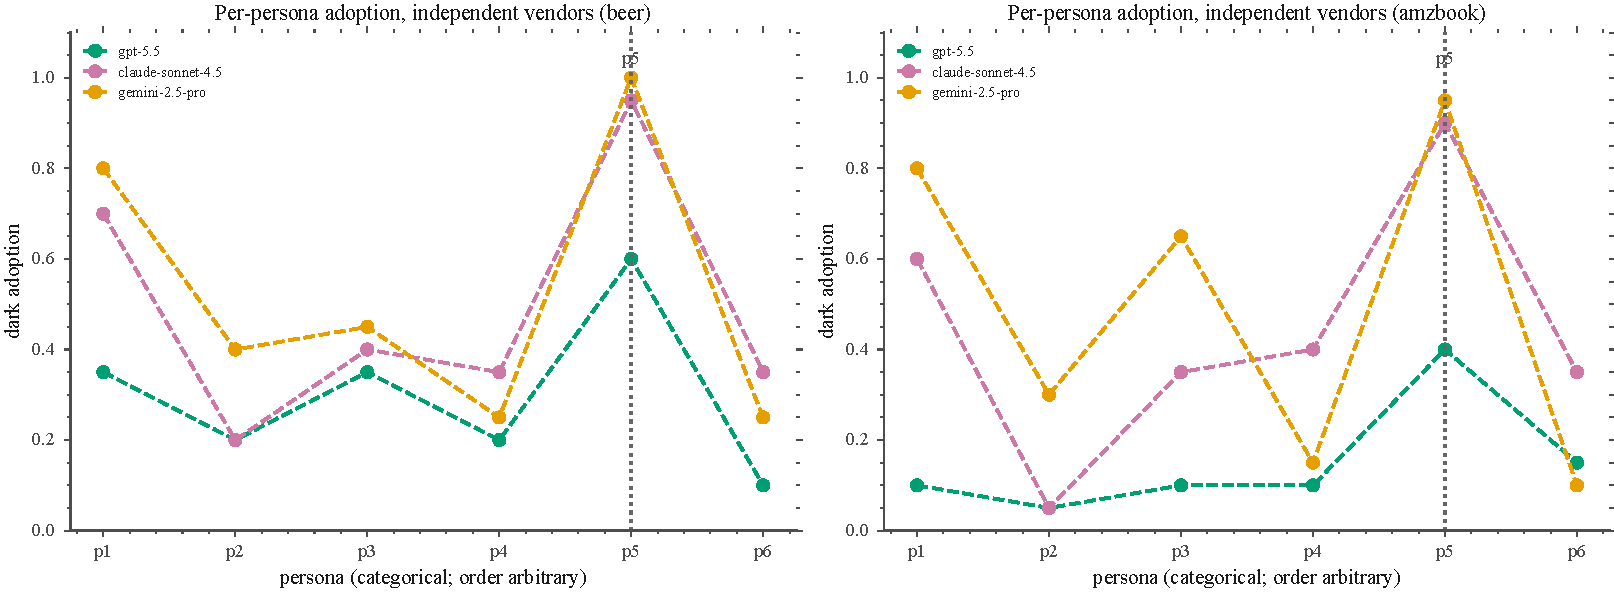
\includegraphics[width=\textwidth]{fig4_rate_vs_ordering}
  \caption{Left: aggregate wrong-advice adoption is model-idiosyncratic (large spread across models).
  Right: the per-persona adoption profile agrees across independent vendors (gpt-5.5, claude, gemini),
  all peaking at the trusting-novice persona (mean pairwise Spearman 0.87 on beer).}
  \label{fig:ordering}
\end{figure*}

The persona \emph{ordering} also agrees across \emph{independent vendors}: on beer, the mean pairwise
Spearman correlation of the six-persona adoption profile across gpt-5.5, claude, and gemini is
\textbf{0.87} (min 0.82)---not one model's prompt noise (Figure~\ref{fig:ordering}, right). We are honest
about the boundary: ordering agreement attenuates at the amzbook frontier (independent-vendor mean 0.50),
because the frontier compresses the \emph{non-top} personas toward the floor, making their sub-ranking
noisy. The robust claim is precisely about the \emph{top} of the ordering---the highest-adopting
persona---which is universal.

\subsection{Panel$\leftrightarrow$human correspondence is unvalidated (honest null)}
Across every configuration we can test, the panel's per-condition axis-1 signal does \emph{not}
significantly track the human anchor's (Spearman on $n=5$ conditions; null under BH for all six models).
On amzbook the correspondence is \emph{degenerate}---the human anchor's per-condition over-dispersion is
near-constant, so the test is uninformative rather than a genuine null. We therefore make \emph{no}
predictive-validity claim; only a powered human study (Section~\ref{sec:e6}) can close this gap.

\section{Discussion}

\paragraph{Panel-model choice has safety consequences.} The field's instinct is that a \emph{better} base
model makes a \emph{better} simulator. For danger-screening, the opposite can hold: the frontier model we
test resists a wrong-advice trap that lower-tier panel models fall into, so a single-frontier-model panel
can under-report a risk \emph{within the panel}. If---a hypothesis for the human study, not a demonstrated
fact---the frontier model is less human-like than a team's actual users, that under-report would carry to
deployment. Either way, ``which LLM should power my synthetic study?'' becomes a first-order methodological
choice, arguing for \textbf{deliberately including lower-tier models} in a screening panel.

\paragraph{Screen for \emph{who}, not \emph{how many}.} Because the persona ordering is robust where the
rate is not, the defensible use of today's panel is to \textbf{surface candidate vulnerable profiles} for
a human study to confirm---a hypothesis-generating signal (``this interface may especially endanger
trusting novices''), not an absolute or validated risk gauge.

\paragraph{A concrete stance in the silicon-sampling debate.} Rather than a blanket ``LLMs (don't)
simulate people,'' we offer a measured, replicated claim: \emph{aggregate} failure-rate signals are
model-dependent and do not transfer across models, while \emph{relative} susceptibility orderings
partially do. That distinction is actionable for anyone building simulated-user tools.

\section{Limitations and Threats to Validity}

\begin{itemize}
  \item \textbf{Synthetic personas are not people}---the central threat. The model-dependence result makes
  it concrete: ``the panel'' is not one thing, so any human-facing claim must name the model. Only the
  human study (Section~\ref{sec:e6}) grounds \emph{which} model, if any, tracks people.
  \item \textbf{The screen is not model-agnostic.} Our evidence shows the aggregate signal does not
  transfer across capability tiers; we do not claim a deployable, model-agnostic detector.
  \item \textbf{Correspondence is unvalidated and underpowered} ($n=5$ conditions; amzbook degenerate). No
  predictive-validity claim is made.
  \item \textbf{Two domains, both binary sentiment.} Other task structures (high-stakes, multi-class,
  generative) are future work.
  \item \textbf{Coercive construct is uncontrolled.} Axis-2 uses a guaranteed-wrong AI (an upper-bound
  stress test); we do not report the dark-vs-placebo contrast, so we do not separate coercive framing from
  ordinary wrong-advice following (immediate follow-up).
  \item \textbf{Item selection uses human reliance variance} (disclosed). Holding items out from threshold
  fitting does not remove selection on the human criterion; a fresh-item human check remains, so we treat
  this as unresolved pending the human study.
  \item \textbf{Persona construct validity.} The most-susceptible persona is prompt-defined to be trusting,
  so its robustness is partly instruction-following; its correspondence to a real human profile is
  untested.
\end{itemize}

\section{Planned Human Validation}
\label{sec:e6}

\emph{This study is designed but not yet run or preregistered.} The one thing synthetic compute cannot buy
is grounding against real people. We have designed a stripped, axis-2-only human study (within-subjects,
$N\approx 40$, Prolific) that would test the paper's two strongest, cross-domain-robust positives against
humans: (H1) a guaranteed-wrong AI interface elicits more wrong-advice adoption than a faithful/placebo
baseline; (H2) a \emph{trusting-novice human index} (high self-reported AI-deference $\times$ low domain
skill) predicts the highest wrong-AI adoption---the human test of Section~\ref{sec:modeldep}; and (H3)
\emph{which} ladder model's panel best tracks the human pattern, with the sharp prediction that a mid-tier
model tracks humans better than the resistant frontier---i.e.\ the most-capable panel model may be the
least human-faithful screener. All outcomes, including nulls, would be publishable bounds on
synthetic-panel validity.

\section{Conclusion}

An interface can fail two ways---by making reliance dangerously uneven, or by coercing uniform trust in a
wrong AI---and teams would like to catch both before an expensive human study. We built a calibrated
synthetic panel to do that triage and found that its danger signal is \textbf{model-dependent}: the
frontier model we test resists the very wrong-advice trap that lower-tier panel models fall for, so the
choice of panel model is itself a methodological decision with safety consequences. What survives that
instability is \emph{which persona} the panel ranks highest: a trusting-novice profile is the
most-susceptible persona for every model on every domain---a robust synthetic invariant whose human
counterpart we have designed a study to test. We offer this as an honest map of where synthetic-user
screening can and cannot be trusted today, and design the human study that would turn a robust
\emph{ordering} into a validated \emph{prediction}.

\begin{acks}
Reproducibility: analysis \texttt{scripts/analysis/axis2\_robustness.py} $\to$
\texttt{results/axis2\_robustness.json}; figures \texttt{scripts/analysis/make\_figures.py}; a decisions
log with preregistration timestamps and audit verdicts accompanies the submission.
\end{acks}

\bibliographystyle{ACM-Reference-Format}
\bibliography{references}

\end{document}
